\subsection{Screens der Blue TOTP Extension}
\label{anh: blue totp ext screens}

\begin{figure}[H]
    \centering
    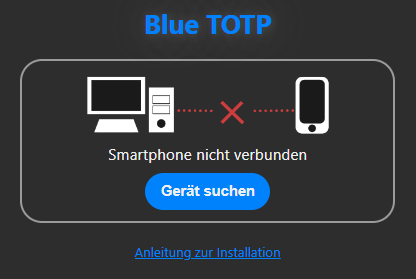
\includegraphics[width=0.5\linewidth]{figures/impl/ext_nicht_verbunden.png}
    \caption[Blue TOTP Extension Home Screen]{Blue TOTP Extension Home Screen. Die Extension aktuell mit keinem Smartphone verbunden und zeigt daher auch nicht die Option zur Einrichtung an.}
    \label{fig: blue totp ext screenshot nicht verbunden}
\end{figure}

\begin{figure}[H]
    \centering
    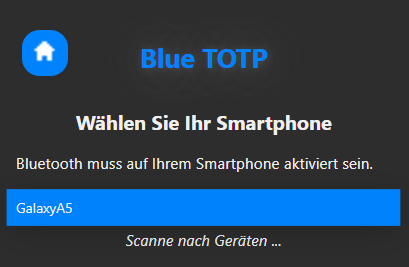
\includegraphics[width=0.5\linewidth]{figures/impl/ext_scan.png}
    \caption[Blue TOTP Extension Scan Screen]{Blue TOTP Extension Scan Screen. Die Extension scannt nach Smartphones mit aktiven Blue TOTP Apps und hat ein Gerät \glqq GalaxyA5\grqq{} gefunden.}
    \label{fig: blue totp ext screenshot scan}
\end{figure}

\begin{figure}[H]
    \centering
    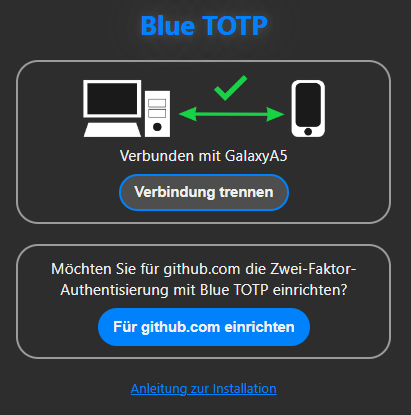
\includegraphics[width=0.5\linewidth]{figures/impl/ext_verbunden.png}
    \caption[Blue TOTP Extension Home Screen (verbunden)]{Blue TOTP Extension Home Screen, der anzeigt, dass die Extension mit dem \glqq GalaxyA5\grqq{} verbunden ist.}
    \label{fig: blue totp ext screenshot verbunden}
\end{figure}

\begin{figure}[H]
    \centering
    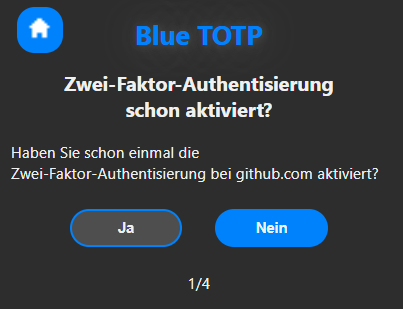
\includegraphics[width=0.5\linewidth]{figures/impl/ext_anleitung_1.png}
    \caption[Blue TOTP Extension Anleitung Screen 1/4]{Blue TOTP Extension Anleitung Screen 1/4. Dieser Screen erfragt, ob der Nutzer bereits die 2FA für die aktuelle Website eingerichtet hat und zeigt dann je nach Antwort eine leicht geänderte Anleitung auf Screen 2/4.}
    \label{fig: blue totp ext screenshot anleitung 1}
\end{figure}

\begin{figure}[H]
    \centering
    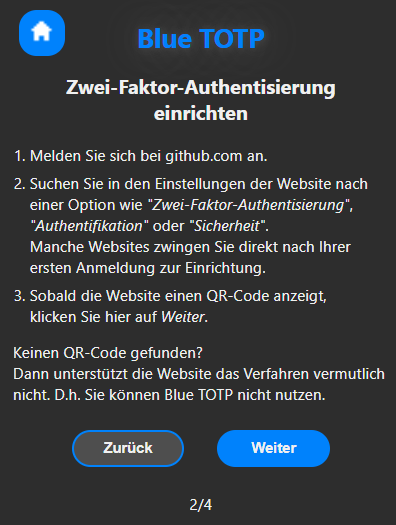
\includegraphics[width=0.5\linewidth]{figures/impl/ext_anleitung_2.png}
    \caption[Blue TOTP Extension Anleitung Screen 2/4]{Blue TOTP Extension Anleitung Screen 2/4. Dieser Screen erklärt dem Nutzer wie er zur 2FA-Einrichtung gelangt. Ziel ist es, dass die Website dem Nutzer den QR-Code anzeigt.}
    \label{fig: blue totp ext screenshot anleitung 2}
\end{figure}

\begin{figure}[H]
    \centering
    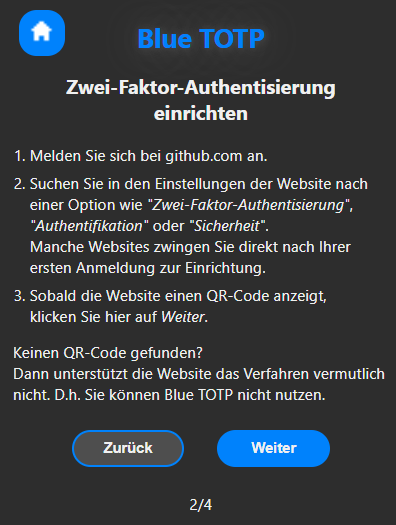
\includegraphics[width=0.5\linewidth]{figures/impl/ext_anleitung_2.png}
    \caption[Blue TOTP Extension Anleitung Screen 3/4]{Blue TOTP Extension Anleitung Screen 3/4. Dieser Screen erfragt den Nutzernamen. Das Eingabefeld ist vorausgefüllt, wenn die Extension den Benutzernamen beim Login mitlesen konnte.}
    \label{fig: blue totp ext screenshot anleitung 3}
\end{figure}

\begin{figure}[H]
    \centering
    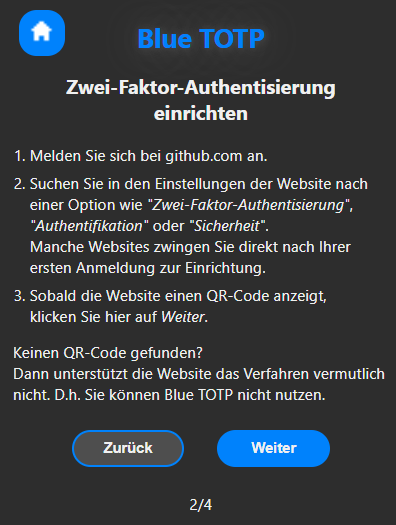
\includegraphics[width=0.5\linewidth]{figures/impl/ext_anleitung_2.png}
    \caption[Blue TOTP Extension Anleitung Screen 4/4]{Blue TOTP Extension Anleitung Screen 4/4. Dieser Screen sagt dem Nutzer, dass er nun mit der Blue TOTP App den QR-Code scannen soll.}
    \label{fig: blue totp ext screenshot anleitung 4}
\end{figure}

\begin{figure}[H]
    \centering
    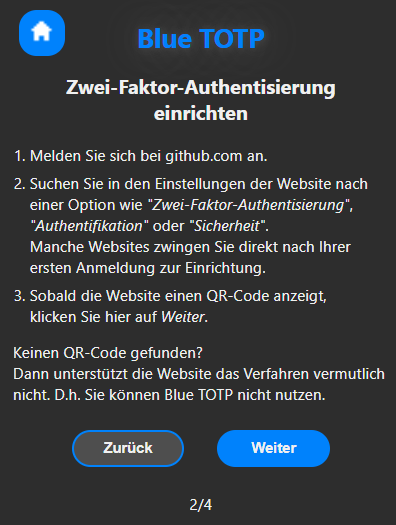
\includegraphics[width=0.5\linewidth]{figures/impl/ext_anleitung_2.png}
    \caption[Blue TOTP Extension Hinweis in Website]{Blue TOTP Extension Hinweis in der Website, der erscheint, wenn der Nutzer das TOTP eingeben muss. Der grün umrandete Bereich ist Ende des TOTP-Eingabeelements. }
    \label{fig: blue totp ext hinweis}
\end{figure}
\newpage